\documentclass[12pt]{article}

\usepackage{sbc-template}

\usepackage{graphicx,url}
\usepackage{pifont} 
\usepackage[square,numbers]{natbib}
\usepackage[brazil]{babel}   
\usepackage{pdfpages}
\usepackage{pgfgantt}
%\usepackage[latin1]{inputenc}  
\usepackage[utf8]{inputenc}  
% UTF-8 encoding is recommended by ShareLaTex

\sloppy

\begin{document} 

\setlength{\voffset}{0cm}
\setlength{\hoffset}{0cm}

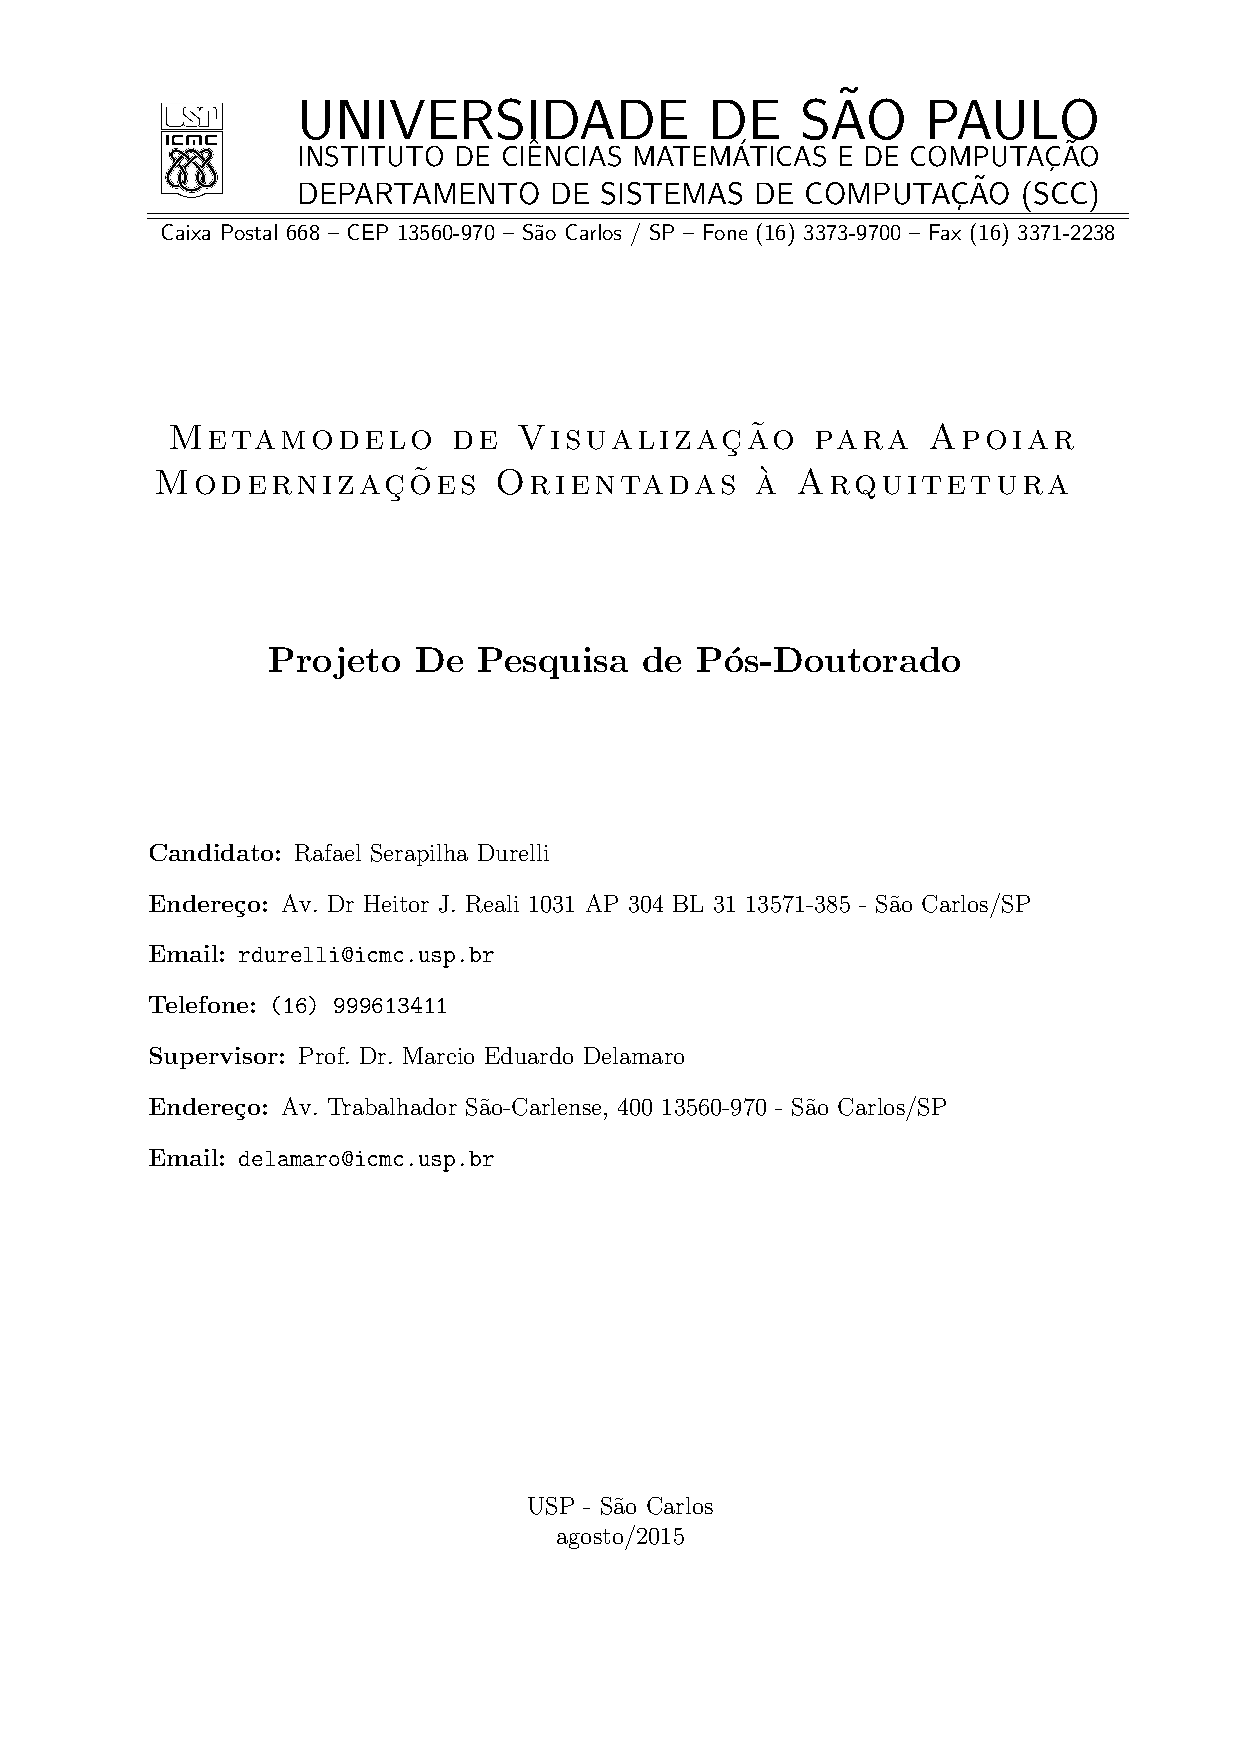
\includepdf[pages=-]{CAPA.pdf}

\begin{resumo}
Manter sistemas legados é uma atividade complexa e custosa para muitas empresas. Uma proposta recente para esse problema é a Modernização Dirigida à Arquitetura (\textit{Architecture-Driven Modernization} - ADM), proposta pela OMG (\textit{Object Management Group}). A ADM consiste em um conjunto de princípios e metamodelos padrões que apoiam a modernização de sistemas utilizando modelos. O \textit{Knowledge Discovery Metamodel} (KDM) é o principal metamodelo da ADM, podendo representar diversos artefatos de um sistema, como código-fonte, arquitetura, interface de usuário, arquivos de configuração e processos de negócio. Embora a ADM e o KDM tenha sido criados para auxiliar o ciclo completo do processo de modernização, observa-se atualmente carência de abordagens que fornecem apoio a partes específicas deste ciclo, fato que indica foco em partes isoladas no lugar do processo como um todo. Além disso, geralmente atividades de modernização são conduzidas sem uma clara especificação do problema existente e da solução almejada. Isto prejudica a análise de impacto da modernização, além de inviabilizar a comparação entre diferentes opções de modernização. Este projeto de pós-doutorado tem o objetivo de propor e implementar uma abordagem de modernização arquitetural, com abrangência de todo o ciclo de modernização, automática e que permita a análise e comparação entre possíveis conjuntos de transformações a serem adotados antes da sua execução. Assim, o engenheiro poderá analisar o cenário de modernização antes de efetivamente realizar a modernização do sistema por intermédio de apoio de representações visuais.
\end{resumo}

\section{Introdução}

\subsection{Contexto}

A partir do momento em que um software começa a ser utilizado, ele entra em um estado contínuo de mudança. Mesmo que tenha sido construído seguindo as melhores técnicas de projeto e codificação existentes, os softwares tendem a se tornarem obsoletos em vistas das novas tecnologias que são disponibilizadas ou em consequência de manutenção que são feitas sem planejamento. Além das correções de erros, as mudanças mais comuns que os software sofrem são migrações para novas arquiteturas, ajustes para mudanças de tecnologias de hardware ou extensões em sua funcionalidade para atender a novos requisitos dos usuários~\cite{Krueger92, SoftwareReuse}

A arquitetura de software é uma das partes mais importantes dentro do ciclo de vida de um sistema de software, pois as decisões tomadas em nível arquitetural possuem impacto direto sobre o sucesso ou fracasso na realização dos objetivos funcionais, de negocio e de qualidade do sistema~\cite{Garcia2009}. Porém, Maffort \textit{et al}.~\cite{Maffort_2013}, explicam que como os modelos arquiteturais possuem um alto nível de abstração, desvios na arquitetura de software surgem facilmente durante o desenvolvimento e manutenção de sistemas de software, tais desvios são definidos na literatura como ``erosão arquitetural''. 

De acordo com Demeyer \textit{et al.}~\cite{Demeyer1}, ``erosões arquiteturais'' causadas pela manutenção de software cresce constantemente, sendo que as soluções não acompanham essa evolução. Esses problemas são resultantes de código-fonte e documentação mal elaborados, além da ausência de técnicas e abordagens para auxiliar a compreensão e visualização do sistema. Segundo Pressman~\cite{Pressman} a atividade de manutenção consome em média 70\% de todo o esforço despendido durante o ciclo de vida de um software. Outro problema é que muitas tarefas de manutenção necessitam de grandes modificações em níveis arquiteturais, as quais são normalmente feitas manualmente e com pouco ou nenhum apoio de recursos de visualização. Fato que aumenta a possibilidade da inclusão de efeitos colaterais em outros módulos do sistema. Além disso, em geral, abordagens de manutenção são iniciadas sem que estejam claros o objetivo e a estratégia a serem utilizadas na sua execução, dificultando a verificação e constatação se o problema foi efetivamente resolvido.

Uma das formas de melhorar a qualidade da arquitetura de software é submetê-la a um processo de reestruturação/refatoração. Esse processo no qual ``transformações'' são realizadas no sistema com o intuito de melhorar sua estrutura sem alterar seu comportamento original~\cite{Canfora2011}. Em 2003 a \textit{Object Management Group} (OMG) criou uma força tarefa para analisar e evoluir os tradicionais processos de reengenharia de software, formalizando-os e fazendo com que eles fossem apoiados por modelos~\cite{OMGADM}. Logo, o conceito tradicional de reengenharia de software começou a mudar e o termo Modernização Dirigida à Arquitetura (\textit{Architecture-Driven Modernization} - ADM) surgiu como uma solução para os problemas de padronização. A ADM é um processo de modernização\footnote{Modernização e reestruturação são dois termos utilizados no contexto deste projeto de forma intercambiáveis} de sistemas legados que utiliza um conjunto de metamodelos para descrever um sistema em diferentes representações arquiteturais~\cite{ADM:OMG}. A ADM preconiza que os processos de reengenharia de software devem seguir os padrões já definidos da Arquitetura Orientada a Modelo (\textit{Model-Driven Architecture} - MDA): \textit{Platform Specific Model} (PSM), \textit{Platform Independent Model} (PIM) e \textit{Computational Independent Model} (CIM). Dessa forma, durante a reestruturação de um sistema são gerados várias instâncias de metamodelos que representam diferentes partes do sistema, como: fluxo de dados, banco de dados, elementos de programação (métodos, classes, tipos de dados, etc.), arquitetura e processos de negócio~\cite{Kleppe:2003, PerezCastillo:2011jo}. 

Em Novembro de 2003, a ADM criou uma \textit{Request-for-Proposal} (RFP) que por sua vez descrevia um conjunto de metamodelos, tais metamodelos são: (i) \textit{Knowledge Discovery Metamodel} (KDM), (ii) \textit{Structured Metrics Metamodel} (SMM) é um metamodelo para representação de métricas e resultados de medições, (iii) \textit{ADM Pattern Recognition} (ADMPR), que facilita a busca de padrões em um software, (iv) \textit{ADM Visualization Specification} (ADMVS), que tem como objetivo representar visualmente metadados de uma aplicação representada em KDM, (v) \textit{ADM Refactoring Specification} (ADMRS), que define maneiras nos quais modelos KDM podem ser usados para refatorar aplicações. É de suma importância destacar que alguns metamodelos encontram-se finalizados e outros ainda não foram nem mesmo discutidos e disponíveis pela OMG e ADM, como por exemplo o ADMVS e ADMRS. De acordo com a OMG, o KDM é o principal metamodelo da ADM. Esse metamodelo contêm um conjunto de pacotes para representar ``todos'' os artefatos de um sistema, por exemplo, com o KDM é possível representar desde de detalhes de baixo nível, como linhas de código, até conceitos abstratos não presentes em uma linguagem de programação, como módulos arquiteturais e processos de negócio. Um pacote importante no contexto deste projeto é o pacote \textit{Structure}, que contêm metaclasses relacionadas com elementos arquiteturais de um sistema.

%Em paralelo, pode-se observar também durante o mapeamento sistemático conduzido~\ref{durelli_systematic_mapping} a carência de abordagens que forneçam apoio adequado e automático a todo o processo de modernização arquitetural. Usualmente as abordagens tem enfoque em partes isoladas do processo de modernização. Por exemplo, são encontradas abordagens que tem enfoque apenas na primeira etapa do processo, que é a mineração de interesses. Algumas mais voltadas à mineração de aspectos~\cite{...}, outras que tem interesse na mineração de padrões~\cite{}, e outras que se preocupam apenas com as transformações~\cite{}. Outras abordagens tem enfoque nas seguintes etapas, que é a modernização. Usualmente durante a modernizações é necessário alterar toda a arquitetura de um sistema, por exemplo, considerando um sistema que não segue uma determina arquitetura, pode-se haver o objetivo de modernizá-lo para o padrão MVC (\textit{Model-View-Controller}). Quando as abordagens possuem enfoque em apenas uma etapa de forma isolada, torna-se difícil obter uma visão completa do sistema, impedindo uma análise mais detalhada e aprofundada a respeito dos problemas arquiteturais existentes no sistema e possíveis soluções.

%Além disso, outra deficiência percebida é a ausência de uma técnica sistemática e padronizada que permita visualizar a arquitetura de um sistema e aplicar um conjunto de transformações para modernizar o sistema. Portanto, muitas tarefas de modernização são iniciadas sem um claro entendimento dos problemas atuais e sem uma visualização precisa das melhorias esperadas após a modernização; fazendo com que não sejam efetivas na solução dos problemas existentes. Contudo, apesar dos importantes avanços no estado da arte feitos por esse trabalho de doutorado e dos trabalhos encontrados na literatura, ainda existe escassez de estudos que identificam e exploram abordagem de modernização arquitetural, completa e automática. Além disso, ainda existem questões em aberto em relação a quais metáforas visuais podem fornecer apoio efetivo durante às atividades de modernização arquitetural de projetos de software.

Um dos problemas que motiva a condução deste trabalho de pós-doutorado é a ausência de um metamodelo de referência com a estrutura adequada para a instanciação das metáforas visuais de apoio às atividades de modernização de arquiteturas de software. Embora a ADM tenha proposta a especificação ADM \textit{Visualization Specification} (ADMVS), até o momento nenhum trabalho ou documento foi disponibilizado pela OMG e ADM. Assim, o candidato pretende deste projeto identificar qual estrutura e informações relevantes são necessárias para que o metamodelo em questão posso instanciar metáforas visuais para apoiar decisões em processos de modernização. Este metamodelo seria uma iniciativa e uma referência em termos de metadados necessárias para instanciar as metáforas visuais para apoiar a análise e decisão em atividades de modernização arquitetural. 

Vale destacar que a ausência de uma referência e um padrão para apoiar a visualização durante o processo de modernização pode ter como resultado o aumento do esforço e consequentemente custo no ajuste e reutilização de outros modelos não padronizados para a instanciação das metáforas visuais. Em linhas gerais, as abordagens de modernização arquiteturais atuais aplicam um conjunto de transformações no sistema a ser modernizado \textit{(incluir refs aqui)}. Em seguida, testes no sistema são aplicados para averiguar se a funcionalidade não foi alterada e se os requisitos arquiteturais foram alcançados \textit{(incluir refs aqui)}. Entretanto, isso não garante que os problemas foram resolvidos.

É importante destacar que este projeto sendo proposto terá colaboração de pesquisas nacional e internacional entre o Instituto de Ciências Matemáticas e de Computação da Universidade de São Paulo - ICMC/USP, a Universidade de Salvador (UNIFACS) e o Institut National de Recherche en Informatique et en Automatique - INRIA/França. Considerando esse cenário, o candidato irá realizar parte das atividades contidas neste plano de pós-doutorado nessas duas instituições. Dessa forma, a realização do presente projeto proporcionará um significativo incremento na formação do bolsista como pesquisador e também aumentará a qualidade das publicações científicas a serem produzidas, o que motiva sua permanência na mesma instituição em que foi conduzido seu doutorado.


\section{Motivação}

As principais motivações deste projeto são:

\begin{enumerate}

\item A escassez de estudos que identificam e exploram quais são as principais metáforas visuais em um projeto de modernização arquitetural. Isto é, quais são as visualizações que permitem visualizar, analisar e resolver desvios arquiteturais de forma efetiva. A ausência de estudos desse tipo dificulta a condução adequada e efetiva de modernizações arquiteturais;

\item ausência de um metamodelo que reúne as principais informações de apoio à análise de desvios arquiteturais em processos de modernização. A maior parte das ferramentas que permitem visualização arquitetural não possuem foco na representação dos desvios, apenas em mostrar os elementos arquiteturais e suas relações, o que também dificulta a condução de processos desse tipo;

\item A inadequabilidade do metamodelo KDM em servir de base para a direta geração de metáforas visuais. Como esse metamodelo é direcionado à representação de artefatos de software e não de elementos gráficos, a geração de metáforas visuais a partir dele resulta em transformações excessivamente complexas e de difícil manutenção. Isso ocorre porque dentro de uma única transformação \textit{T}, haveria conhecimento relacionado a elementos de código-fonte, que precisam ser lidos do KDM, e elementos gráficos, que precisariam ser representados visualmente.
\end{enumerate}
 

\section{Objetivos}

O objetivo mais amplo deste projeto é fazer com que modernizações arquiteturais possam ser feitas de forma mais efetiva. Para que esse objetivo seja alcançado, os seguintes objetivos específicos devem ser atingidos:

\begin{enumerate}
\item Identificar as metáforas visuais que fornecem apoio efetivo durante projetos de modernização arquitetural, de forma a facilitar a análise e exploração dos desvios arquiteturais de um sistema;

\item Criar um Metamodelo de Visualização Arquitetural (MVA) que reúne as metaclasses mais adequadas para a representação não só de elementos arquiteturais mas também de desvios que ocorrem entre esses elementos. Assim como ocorre com o metamodelo SMM, o MVA que será desenvolvido neste projeto possui bastante relação com o KDM, podendo, inclusive, referenciar algumas de suas metaclasses. Assim, um dos objetivos é que esse MVA possa ser utilizado como iniciativa para o metamodelo de visualização que está sendo atualmente desenvolvido pela OMG (documento de visualização da omg);

\item Fazer com que as transformações de modelo tornem-se mais claras e de manutenção mais facilitada. Isso deverá ser obtido pois pretende-se dividir as transformações em dois passos: i) Transformação do KDM para MVA e depois do MVA para as metáforas visuais;

\item Encorajar desenvolvedores de ferramentas de modernização a utilizarem o KDM e o MVA proposto como base dentro de suas ferramentas.

\end{enumerate}


%Neste projeto de pós-doutorado, o objetivo é o desenvolvimento de uma abordagem de modernização, completa e automática, que permita visualizar o impacto positivo e negativo que determinado conjunto de transformação tem no sistema, antes de efetivamente conduzir o processo. Assim, o engenheiro poderá analisar o cenário de modernização antes de efetivamente realizar a modernização do sistema por intermédio de apoio de representações visuais.

%Para isso, inicialmente, o engenheiro de modernização deve obter um panorama dos problemas atuais do sistema, o que será feito por meio de uma nova abordagem de mineração com o foco em identificar elementos de código que implementam os conceitos da arquitetura alvo. As abordagens atuais de mineração tem enfoque na identificação de tipos específicos de interesses, não sendo eficazes na identificação de tipos variados. Dessa forma, pretende-se evoluir duas ferramentas (SourceMiner e CCKDM) já desenvolvidas por colaboradores deste projeto~\cite{source_miner_glauco, daniel_san_journal} no sentido de permitir que elas possam minerar elementos de código que implementam os conceitos arquiteturais.

%A análise da arquitetura será apoiada pelo uso combinado de um conjunto de metáforas visuais instanciadas a partir do metamodelo proposto. As metáforas poderão ser ajustadas a partir dos filtros disponíveis na interface gráfica de forma que nem todos os elementos armazenados no metamodelo sejam representados visualmente na tela. Isto possibilita a configuração do cenário visual de acordo com o objetivo da atividade de compreensão da arquitetura realizada. Por exemplo, será possível configurar os filtros para que seja dada ênfase às características de determinado modelo arquitetural alvo. Assim, será possível ajustar as metáforas visuais para indicar módulos do sistema que tenham mais coesão e menos acoplamento com outros módulos; ou se o sistema analisado está aderente a um conjunto de regras de uma determinada arquitetura ou ainda para indicar o grau de modularização de determinados interesses transversais como persistência e segurança.

%Depois do ajuste das metáforas visuais de acordo com as características esperadas para uma possível arquitetura alvo, poderá ser feita a análise do que deverá ser feito para transformar o sistema estudado. Isto será possível pelo fato de cada modelo arquitetural alvo possuir um conjunto de metáforas visuais indicado para sua representação e também um conjunto de filtros que podem ser utilizados para apoiar a análise. Isto apoiará a execução das transformações que visam a atender aos requisitos que foram especificados pelo modernizador. Os modelos arquiteturais recomendados pela abordagem poderão ser comparados quantitativamente. Desta forma, o nível de atendimento da arquitetura recomendada 1 atente a 70\% do modelo arquitetural alvo, enquanto que o modelo arquitetural recomendado 2 atende a 90\% do modelo arquitetural alvo. Depois de analisar os modelos arquiteturais, o modernizador poderá escolher pelo mais adequado e assim a abordagem irá efetivamente modernizar o sistema. 

\subsection{Experiência do Grupo com ADM e KDM}

Durante o projeto de doutorado do candidato, Bolsa de Doutorado, Processo N. 2012/05168-4, juntamente com parcerias, foram definidos e elaborados um conjunto de soluções para auxiliar e colaborar com a ADM e seus metamodelos: por exemplo, em~\cite{dani_san_tool, dani_san, daniel_san_journal} o candidato juntamente com uma parceria desenvolveram técnicas de mineração de interesse transversal com a utilização do metamodelo KDM. Em ~\cite{Santos_2014, santo_wmod} o candidato com a colaboração de outro pesquisador criaram um perfil para permitir que o metamodelo KDM desse total suporte ao Paradigma Orientado a Aspecto (POA) durante a modernização de sistemas, uma iniciativa para utilizar o metamodelo SMM também foi desenvolvida~\cite{honda_dissertacao}. 

Além disso, foi identificado pelo candidato uma ausência de catálogos de refatorações adaptados para o metamodelo KDM~\cite{durelli_systematic_mapping} - a vantagem seria que qualquer catalogo adaptado para o KDM seria independente de plataforma e de linguagem de programação - aumentando assim o reuso e a interoperabilidade entre diversas ferramentas de modernização. Dessa forma, o candidato desenvolveu um conjunto de refatorações e um ambiente totalmente automatizado para auxiliar à aplicação de refatorações para o metamodelo KDM~\cite{durelli_catalogo, durelli_VEM_ferramenta}. Durante um mapeamento sistemático conduzido~\cite{durelli_systematic_mapping} pôde-se observar na literatura a carência de estudos que definem soluções para especificar refatorações para o KDM. De acordo com a OMG, sem a adequada representação de refatorações no contexto do metamodelo KDM, a realização e a reutilização de uma refatoração pode se tornar uma atividade propensa a erros e difícil. Dessa forma, o candidato de definiu um metamodelo para persistir metadados de refatorações, ou seja, o principal objetivo desse metamodelo é ser uma iniciativa e uma proposta para a especificação ADM \textit{Refactoring Specification} (ADMRS). Esse metamodelo permite a representação de refatorações de granularidade fina e grossa, porém, ainda respeita a independência de linguagem e plataforma uma das principais características e vantagens dos metamodelos definidos pela OMG e ADM. 

\section{Organização da Proposta}

O restante deste projeto está organizado da seguinte forma. Na Seção~\ref{sec:fundamentacao_teorica} a fundamentação teórica é apresentada, dando especial atenção ao metamodelo KDM e visualização de software no contexto da ADM e KDM. Na Seção~\ref{sec:proposta_de_trabalho} a proposta do projeto é apresentado. Essa seção é dividida em cinco subseções (\textit{i}) Desafios de Pesquisa com Relação ao Projeto; (\textit{ii}) Plano de Trabalho e Cronograma; (\textit{iii}) Materiais e Métodos; (\textit{iv}) Avaliação e disseminação; (\textit{v}) Resultados Relacionados. Por fim, a Seção~\ref{sec:colaboracoes} apresenta os pesquisadores que irão colaborar para a realização do projeto aqui proposto.

\section{Fundamentação Teórica}\label{sec:fundamentacao_teorica}

\subsection{\textit{Knowledge Discovery Meta-model} (KDM)}

De acordo com a OMG o metamodelo \textit{Knowledge Discovery Meta-model} (KDM) é o metamodelo mais importante definido pela ADM. Esse metamodelo pode ser utilizado para representar artefatos de software, seus elementos, associações, e ambientes operacionais. O KDM tem como principal objetivo permitir que engenheiros de software criem ferramentas para auxiliar a modernização de software que sejam independente de plataforma e linguagem~\cite{PerezCastillo:2011jo, ADMCHAPTERR}. Além disso, o KDM facilita projetos que envolvem sistemas de software existentes, assegurando a interoperabilidade e troca de dados entre as ferramentas fornecidas por diferentes fornecedores. 

Um problema tradicional facilmente identificado em várias ferramentas que lidam com a reengenharia de software é que tais ferramentas analisam diversos artefatos de um determinado software (por exemplo, código-fonte, banco de dados, \textit{scripts}, etc.) para obter conhecimentos explícitos com o intuito de realizar transformações/refatorações. Como consequência cada ferramenta gera e analisa tais conhecimentos de forma implícita, ou seja, os conhecimento gerados são restritos à uma especifica linguagem de programação, e/ou a uma plataforma. Como resultado tais restrições podem criar dificuldades com relação a interoperabilidade entre diferentes ferramentas. Dessa forma, o KDM fornece uma estrutura que facilita a troca de dados entre as diversas ferramentas. Além disso, a estrutura do KDM fornece meios de especificar artefatos físicos e lógicos de um determinado sistema. Consequentemente, todas as técnicas/abordagem/ferramentas que utilizam o KDM como entrada podem ser consideradas independente de plataforma e linguagem, aumentando assim, a interoperabilidade e o reúso. Em 2012 o KDM tornou-se um padronização \textit{International Standards Organization} (ISO)~\cite{KDM:specification} que facilita a troca de dados entre diversas ferramentas. O KDM é definido via \textit{Meta-Object Facility} (MOF)~\cite{MOF}. Além disso, o KDM estabelece o formato de troca de dados via XML \textit{Metadata Interchange} (XMI).

O KDM possui o objetivo de cobrir um amplo escopo, para abranger um conjunto grande e diversificado de aplicações, plataformas e linguagens de programação~\cite{KDM:specification, PerezCastillo:2011jo}. Um dos principais objetivos do KDM é fornecer a capacidade de troca de metadados entre diversas ferramentas e, assim, facilitar a cooperação entre fornecedores para integrar e aumentar a interoperabilidade de diferentes abordagens, técnicas, algoritmos, etc. A fim de alcançar essa interoperabilidade e, especialmente, a integração de informações sobre diferentes facetas de um determinado sistema a partir de múltiplas ferramentas, o KDM define vários níveis de conformidade, aumentando assim a probabilidade de que duas ou mais ferramentas apoiaram o mesmo metamodelo. Além disso, o KDM também é estruturado de forma modular, seguindo o princípio da separação de interesse, com a capacidade de representar partes heterogêneas de um sistema. A separação de interesses no contexto do metamodelo KDM são alcançadas por meio de pacotes, como apresentado na Figura~\ref{kdm:domain}. Cada pacote está em um nível de conformidade e possui o objetivo de definir um ponto de vista arquitetural do sistema. Em outras palavras, cada pacote do KDM constitui uma determinada ontologia para descrever e representar a grande maioria dos artefatos de sistemas de software existentes. Por exemplo, os pacotes \texttt{Code} e \texttt{Action} definem metaclasses para representar o código-fonte de um sistema, tais como, variáveis, procedimentos/métodos/funções, chamadas para procedimentos/métodos/funções. Similarmente o pacote \texttt{Structure} contêm metaclasses para representar elementos arquiteturais do sistema, tais como, componentes, camadas, sub-componentes, etc. O pacote \texttt{Conceptual} possui  metaclasses para definir regras de negócio do sistema.

\begin{figure}[htb]
 \centering
 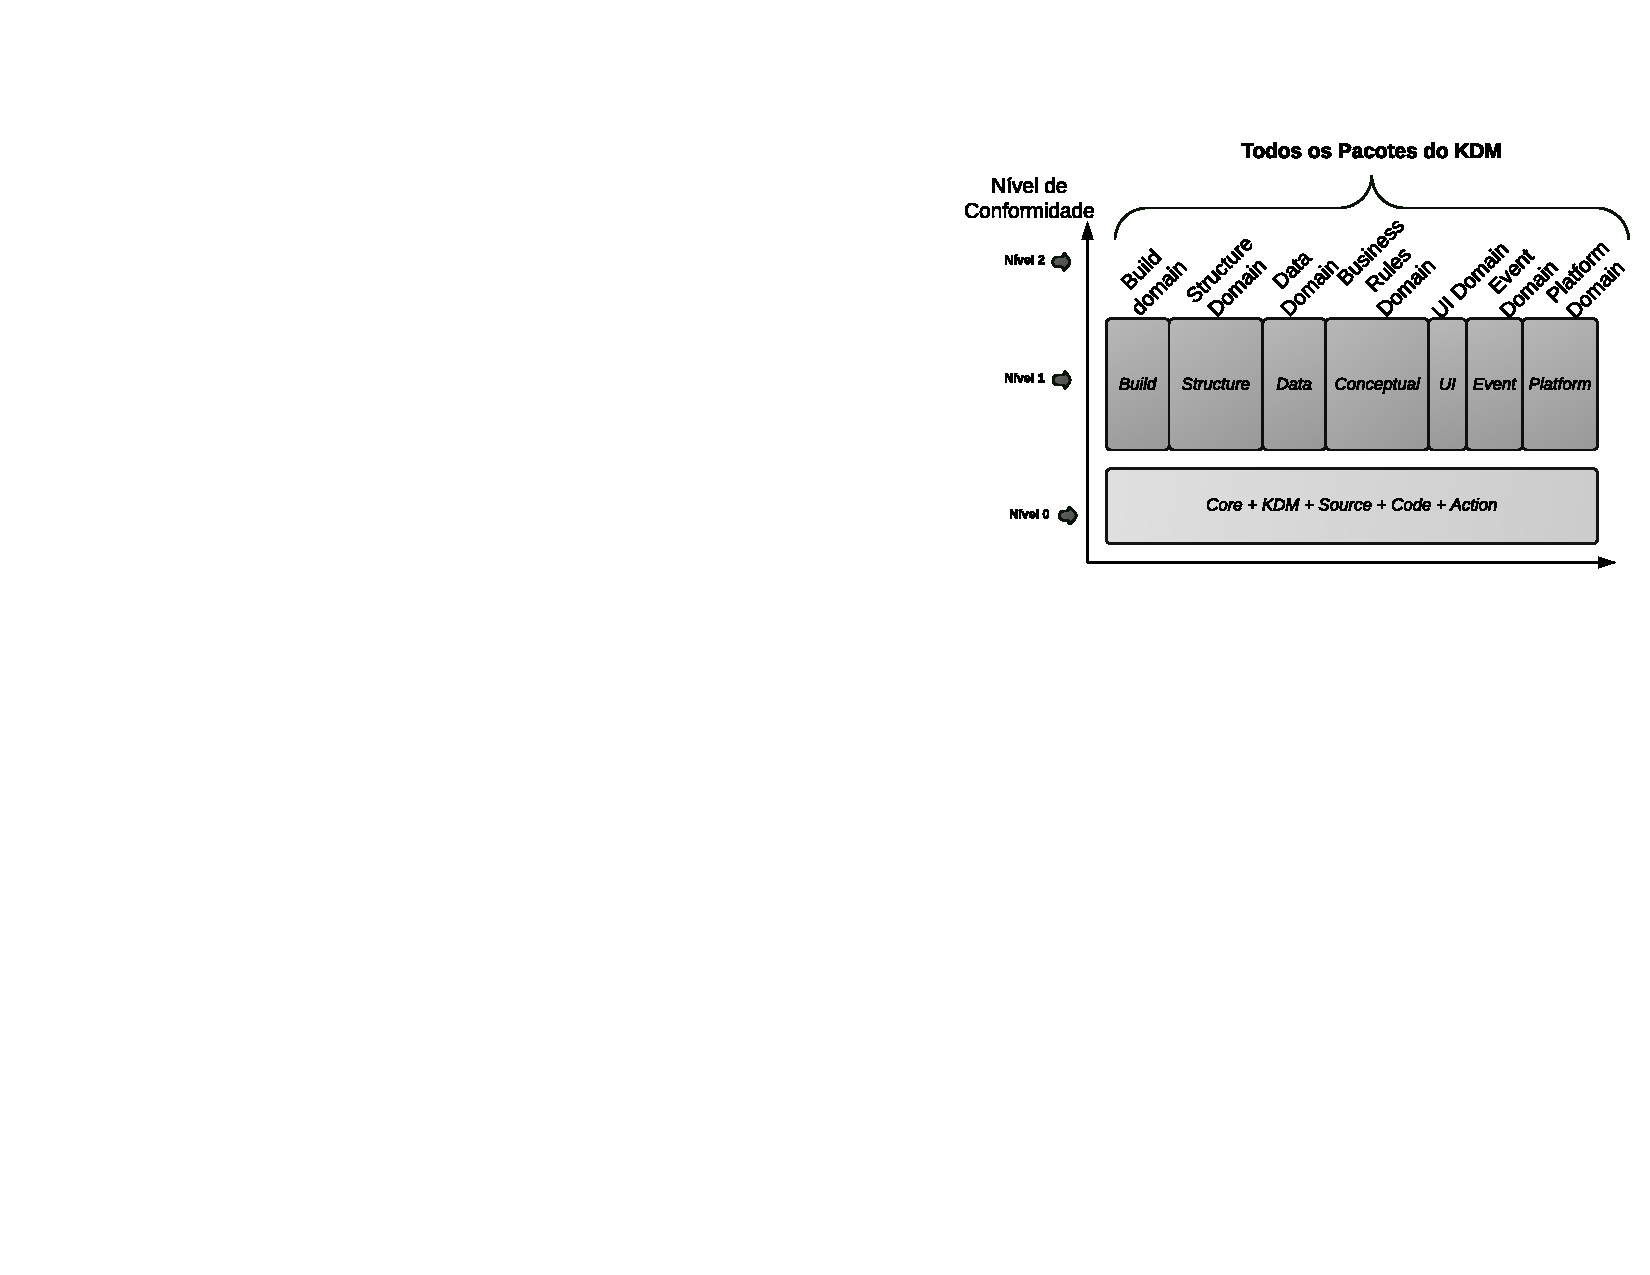
\includegraphics[scale=1]{kdmLevels_pacotes.pdf}
 \caption{Pacotes e nível de conformidade do metamodelo KDM.}
 \label{kdm:domain}
\end{figure}

Da perspectiva de um engenheiro de software, essa separação de interesse do KDM, por meio de pacote, significa que o engenheiro só precisa se preocupar com os pacotes do KDM que considerar necessários para as suas atividades de modernização, por exemplo, uma determinada abordagem pode necessitar apenas do pacote \texttt{Code} e \texttt{Action}, enquanto uma outra abordagem utilize apenas o pacote responsável por definir elementos arquiteturais. Se essas abordagens forem evoluídas ao longo do tempo e necessitarem de outros pacotes do KDM, os respectivos pacotes podem ser adicionado ao repertório da abordagem/ferramenta, conforme necessário.

Como um dos principais objetivos deste projeto é a definição de todo o processo de modernização arquitetural o pacote \texttt{Structure} do metamodelo KDM é apresentado com maiores detalhes. Este pacote, \texttt{Structure} contêm metaclasses que representam componentes arquiteturais de sistema de software existentes, como subsistemas, camadas, componentes, etc. Esse pacote define um ponto de vista arquitetural para um domínio estrutural. As visões de arquitetura com base no ponto de vista definido pelo pacote~$\mathtt{Structure}$ representam a forma como os elementos estruturais do sistema de software estão relacionados com os módulos definidos em código, que correspondem ao pacote~$\mathtt{Code}$. Um trecho do pacote~$\mathtt{Structure}$ é mostrado na Figura ~\ref{fig:structureModel} como um diagrama de classes.

O modelo~$\mathtt{Structure}$ possui uma coleção de elementos estruturais, como pode ser visto na Figura~\ref{fig:structureModel} \ding{202}, isso é representado por meio de uma associação. A metaclasse~$\mathtt{SoftwareSystem}$ fornece um ponto de encontro para todos os pacotes do sistema direta ou indiretamente através de outra associação chamada de~$\mathtt{AbstractStructureElement[0..*]}$. Os pacotes podem ainda ser agrupados nas metaclasses~$\mathtt{SubSystem}$,~$\mathtt{Layer}$,~$\mathtt{Component}$ and~$\mathtt{ArchitectureView}$.


\begin{figure}[h]
 \centering
 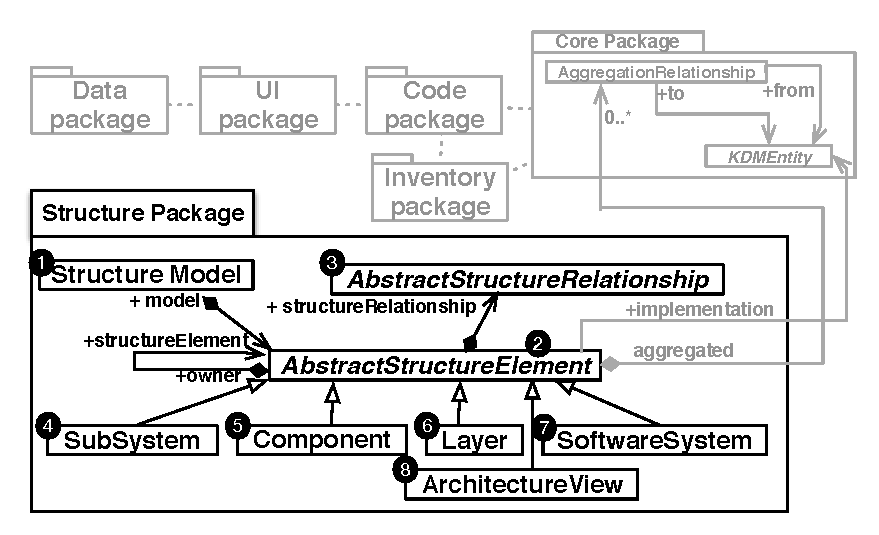
\includegraphics[scale=0.8]{StructurePackageFigure.pdf}
 \caption{Diagrama de classe do Pacote \texttt{Structure}.}
 \label{fig:structureModel}
\end{figure}

A metaclasse~$\mathtt{AbstractStructureElement}$ (conforme a Figura~\ref{fig:structureModel} \ding {203}) representa uma parte arquitetural, relacionada com a organização do sistema de software existente em módulos e possui quatro associações. A primeira associação representa os elementos pertencentes ao modelo e é chamada de $\mathtt{structureElement}$ $\mathtt{:AbstractStructureElement[0..*]}$. Em seguida, há a associação~$\mathtt{structureRelationship}$ $\mathtt{:AbstractStructureRelationship[0..*]}$, ela é usada para representar todas os relacionamentos em nível arquitetural. A associação $\mathtt{aggregated:}$ $\mathtt{AggregatedRelationship[0..*]}$ representa uma relação abstrata entre dois elementos do KDM, dentro dela é possível definir relações concretas. A última associação da metaclasse~$\mathtt{AbstractStructureElement}$ é o~$\mathtt{implementation:KDMEntity[0..*]}$. Esta associação é usada para especificar os elementos computacionais (do pacote~$\mathtt{Code}$, ou seja, $\mathtt{Package}$, $\mathtt{ClassUnit}$, $\mathtt{InterfaceUnit}$, etc) que representam o elemento estrutural. 


Na Figura~\ref{fig:kdm_structureExample} é descrita uma possível arquitetura alvo mostrada para ilustrar como o KDM pode ser utilizado para representar elementos arquiteturais. Nota-se que esta figura está dividida em três níveis para ilustrar como o pacote~$\mathtt{Structure}$ está relacionado com o pacote~$\mathtt{Code}$. O nível mais baixo representa o código-fonte, artefatos físicos. L1 e L2 representam pacotes em código-fonte - cada ``caixa'' dentro dos pacotes representa as suas classes e interfaces, também é possível perceber que essas classes e interfaces são relacionados uns com os outros de alguma maneira. No meio há metaclasses do pacote~$\mathtt{Code}$, o que significa que as instâncias dessas metaclasses são usadas para representar os artefatos de baixo nível, ou seja, instâncias de~$\mathtt{Package}$ são usadas para representar L1 e L2 e instâncias de~$\mathtt{ClassUnit}$ e~$\mathtt{InterfaceUnit}$ são usados para representar as classes e interfaces, respectivamente. Finalmente, no nível superior a arquitetura é mostrada. Todos os elementos arquiteturais são representados com a seguinte padronização: [metaclasse:nome]. A arquitetura alvo é apresentada e dividida da seguinte forma: no ponto mais alto de abstração há um~$\mathtt{SoftwareSystem}$ ($\mathtt{S1}$) \ding {202}, que é dividido em duas camadas, ~$\mathtt{Layer}$~$\mathtt{L1}$ \ding {203} e ~$\mathtt{Layer}$~$\mathtt{L2}$ \ding {204}. Tais camadas representam elementos arquiteturais correspondentes aos pacotes L1 e L2 representadas no nível mais baixo. A~$\mathtt{Layer}$~$\mathtt{L1}$ pode acessar os elementos da~$\mathtt{Layer}$~$\mathtt{L2}$, essa restrição \aspas{pode acessar} é representada pela metaclasse~$\mathtt{AggregatedRelationship}$ \ding {205}. Além disso, a~$\mathtt{Layer}$~$\mathtt{L2}$ contém dois componentes,~$\mathtt{C1}$ \ding {206} e~$\mathtt{C2}$ \ding {207}. Finalmente, o~$\mathtt{Component}$~$\mathtt{C1}$ fornece recursos através de uma interface para o~$\mathtt{Component}$~$\mathtt{C2}$.

\noindent \begin{minipage}{.40\textwidth}
	\centering
	% Requires \usepackage{graphicx}
	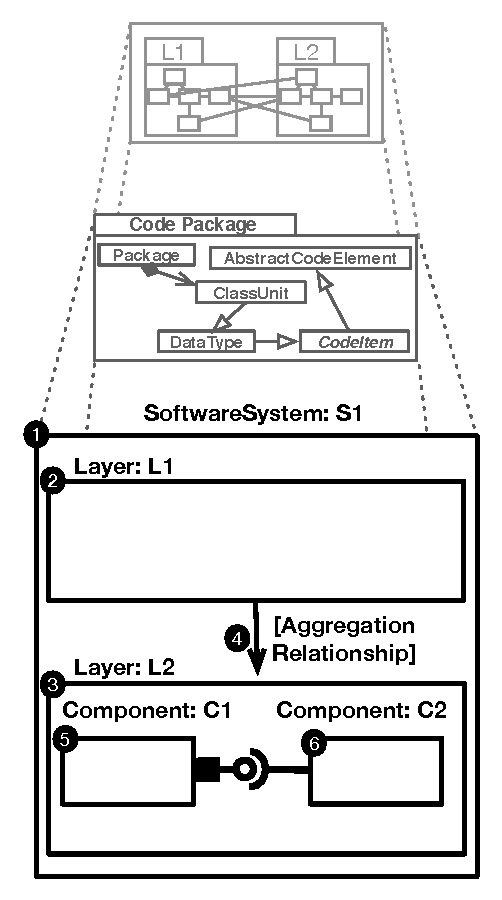
\includegraphics[scale=0.65]{StructureExample}
	\captionof{figure}{Uma possível arquitetural de um sistema.}
	\label{fig:kdm_structureExample}
\end{minipage}\hfill
\begin{minipage}{.64\textwidth}
	\centering
	% Requires \usepackage{graphicx}
	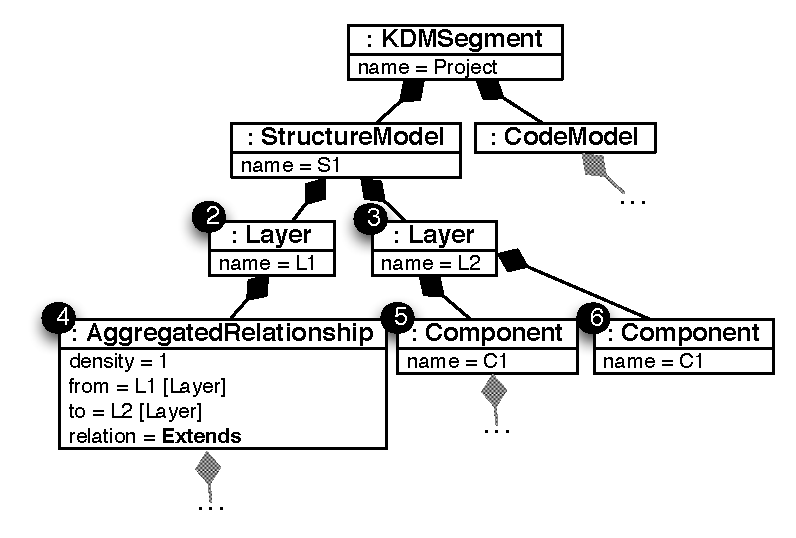
\includegraphics[scale=0.65]{StructureKDMINstance}
	\captionof{figure}{Instância KDM correspondente a Figura~\ref{fig:kdm_structureExample}}
	\label{fig:kdm_instance_StructureExample}
\end{minipage}

\subsection{Visualização de Software no Contexto da ADM e KDM}

Como salientado anteriormente o KDM é um metamodelo que pode ser utilizado para definir desde representações especificadas de um sistema (elementos estruturais e comportamentais de código-fonte) até representações abstratas de um sistema (abstrações arquiteturais, regras de negócio, banco de dados, etc). No entanto, até o momento, existe uma carência de padronizações para auxiliar a definir como visualizar todas as representações do metamodelo KDM, ou seja, como representar visualmente todas as camadas do metamodelo KDM. Dessa forma, usualmente os desenvolvedores precisam que criar suas próprias soluções ferramentais e determinar o que, e como deverá ser visualizado no metamodelo do KDM. Como resultado, tais ferramentas tendem a diminuir a interoperabilidade e a coerência durante a visualização e apresentação de informações para os usuários dessas ferramentas. Uma definição adequada para ``visualização'' no contexto da ADM e KDM é a seguinte: ``Visualização é o processo para representar um determinado sistema como um conjunto de imagens para auxiliar na compreensão de como o sistema está implementado, com o intuito de identificar falhas e erros de projeto''~\cite{ADM:OMG}.

A visualização é um importante meio de compreensão e é fundamental para apoiar a construção de um modelo mental ou uma imagem mental a respeito de alguma representação visual~\cite{spence2014information}. Visualizar é uma atividade cognitiva, apoiada por representações visuais externas através das quais se constrói uma representação mental interna do cenário visual observado~\cite{spence2014information, ware2012information}. No processo de visualização, dados são transformados em imagem. A imagem, por sua vez, é interpretada pelo ser humano. A interpretação de uma imagem pode conduzir à descoberta de informação a partir do que foi codificado graficamente. Isto fecha o ciclo da visualização que tem o objetivo de permitir que informação relevante seja obtida a partir de um conjunto de dados~\cite{source_miner_glauco}. 

Uma visão é uma representação visual de um conjunto de dados. A análise de conjuntos de dados complexos tipicamente requer múltiplas visões, cada uma revelando um aspecto diferente dos dados sob análise~\cite{Boukhelifa_2003}. Este é o caso em engenharia de software, pois uma única visão não necessariamente apoiará a compreensão efetiva dos dados nela representados~\cite{Storey_2006}. Múltiplas visões incentivam a construção de conhecimento mais aprofundado a respeito dos dados analisados e evitam interpretações distorcidas que poderiam emergir de uma única visão~\cite{Ainsworth_1999}. A Figura XX apresenta uma adaptação do modelo Card ~\cite{source_miner_glauco} para a obtenção de um modelo de referência para visualização de informações baseada em múltiplas visões. Múltiplas visões devem ser concebidas de forma consistente para que seja viável a coordenação e integração entre elas. Visões (e formas visuais) devem ser complementares entre si. Um subconjunto de visões deve ser selecionado para uso coordenado durante execução de uma determinada atividade de análise de dados~\cite{WangBaldonado_2000}. A exploração interativa das visões deve ocorrer para que sejam descobertas informações e relacionamentos que se fossem avaliados da forma tradicional permaneceriam ocultos. Um exemplo de ambiente que aplica estes conceitos é o SourceMiner que é um ambiente interativo baseado em múltiplas visões~\cite{source_miner_glauco}. 

No contexto deste projeto, o conjunto de dados está relacionado à modernização arquitetural e o modelo mental construído a partir das representações de um ambiente interativo baseado em múltiplas visões teria o objetivo de tornar mais efetiva a análise de cenários de modernização arquitetural e consequentemente decisões mais fundamentadas nestes cenários. 

Neste contexto, pode-se argumentar que a definição de uma padronização de visualização de software para a ADM e KDM iria beneficiar os modernizadores de software pois aumentaria a interoperabilidade e a coerência durante a visualização e apresentação de informações de um determinado sistema. Além disso, essa padronização poderia também auxiliar modernizadores a visualizar falhas e erros  de forma dinâmica antes da aplicação de refatorações em sistemas que estão em conformidade ao metamodelo KDM. É importante destacar que sem uma forma padronizada para visualizar todas as visões conceituais de um sistema representado utilizando o metamodelo KDM, modernizadores podem ignorar ou até mesmo esquivar de problemas que precisam ser solucionados nesses sistemas. 

Dessa forma, ignorar a visualização de sistemas prejudica possíveis análises e esforços de planejamentos associados com iniciativas de modernizações, como é o caso da ADM e KDM. Assim, é de suma importância definir um conjunto/processo de visualizações de software para o contexto da ADM e KDM. Tais visualizações utilizariam como base o metamodelo KDM, e criariam um conjunto de representações visuais do sistema - o que resultaria em um conjunto de visualizações de software independente de plataforma e de linguagem de programação. Além disso, como o KDM permite a representação de vários artefatos presentes em sistemas legados os conjuntos de visualizações deveriam permitir a visualização desde artefatos específicos (elementos de código-fonte e elementos comportamentais) até artefatos abstratos (elementos arquiteturais e elementos de regra de negócio). Também pretende-se que tais visualizações mostrem os efeitos que um sistema teve após a aplicação de um conjunto de refatorações, assim, modernizadores podem decidir qual a melhor solução durante a atividade de modernização de software.

\section{Proposta de Trabalho}\label{sec:proposta_de_trabalho}

O objetivo é o desenvolvimento de uma abordagem de modernização arquitetural completa e automática que permita que um engenheiro de modernização possa especificar, visualizar e modernizar um determinado sistema para um modelo arquitetural alvo. Posteriormente, o engenheiro pode verificar o grau de atendimento a determinadas transformações relacionadas aos requisitos arquiteturais desejados. Isto é, o engenheiro terá a possibilidade de utilizar visualizações que realmente apoiam as decisões durante todo o processo de modernização. Um modelo arquitetural alvo será especificado pelo engenheiro de software e transformações serão feitas automaticamente depois que o engenheiro optar pelo conjunto mais adequado.

No contexto deste projeto, modelos arquiteturais alvos são possíveis soluções arquiteturais para serem realizadas no sistema legado que possivelmente resolverão os problemas atuais do sistema ou farão com que o sistema tenha melhores níveis de manutenibilidade, reusabilidade e extensibilidade. Exemplos de modelos arquiteturais alvos são: o padrão MVC (\textit{Model-View-Controller}), oSGI (\textit{Open Services Gateway Initiative}), camadas, componentes, SOA (\textit{Service-Oriented Architecture}), etc.

Na Figura~\ref{fig:approach_steps} encontram-se os passos da abordagem deste projeto. Nota-se que essa figura dividida em camadas. Na camada [A] são apresentadas os passos a serem realizadas pelo engenheiro de modernização que utilizará a abordagem; na camada [B] são apresentadas as telas que representam o apoio computacional que será desenvolvido; e na camada [C] são apresentadas os passos internas do apoio computacional.

\begin{figure}[htb]
 \caption{Passos da Abordagem Proposta. FIGURA AINDA NÃO FINALIZADA}
 \label{fig:approach_steps}
 \centering
 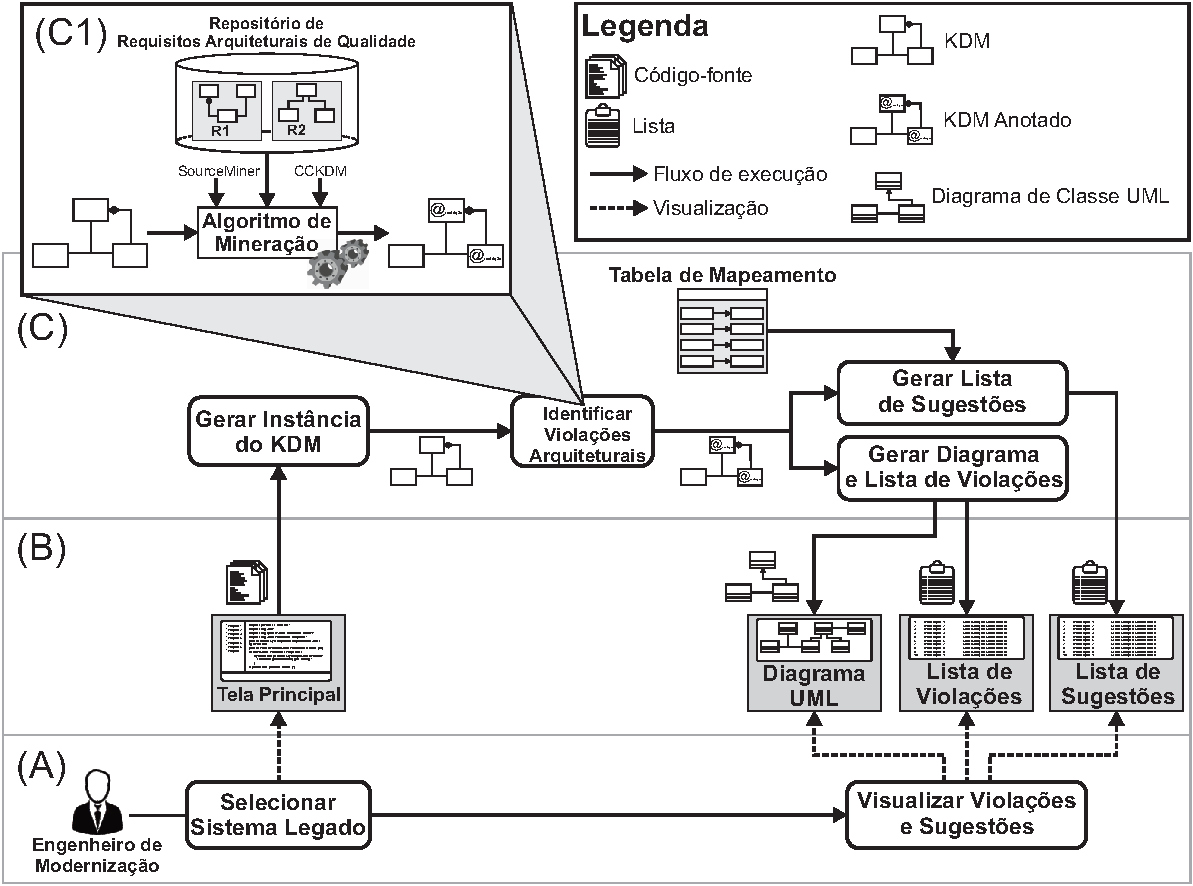
\includegraphics[scale=0.77]{abordagemSteps.pdf}
\end{figure}

O primeiro passo da abordagem consiste em selecionar o sistema legado a ser modernizado (Figura~\ref{fig:approach_steps} (a)). Esse passo será realizado na tela principal do ambiente de desenvolvimento Eclipse\footnote{https://eclipse.org/home/index.php} onde o engenheiro está visualizando o código-fonte do sistema legado, como visualizado na camada [B]. 

Após a escolha do sistema legado a ser modernizado, o próximo passo, denominado ``Gerar instância do KDM'' é executada, como observado na camada [C]. O objetivo desse passo é gerar uma instância do metamodelo KDM que representa todos os artefatos do sistema legado, para tal, o \textit{framework} MoDisco será utilizado.

Após a obtenção da instância do sistema em KDM, o engenheiro de software irá trabalhar com uma linguagem específica de domínio para especificar os requisitos arquiteturais de qualidade desejados. A sintaxe dessa linguagem ainda não foi definida, porém, a princípio ele terá elementos/palavras-chaves que sejam representativos do domínio de modernização. Dessa forma, nesse passo, por exemplo, o engenheiro poderá especificar por meio da linguagem específica de domínio que o sistema legado precisa seguir o modelo arquitetural alvo MVC, compontes, SOA, etc.

Em seguida o passo, denominado ``Identificar Violações Arquiteturais'', é executado. Este passo tem como objetivo identificar e obter uma panorama atual do sistema legado a ser modernizado, maior detalhamento desta etapa é apresentado na camada C1 da Figura~\ref{fig:approach_steps}. Neste passo será desenvolvida e/ou estendida técnicas de mineração~\cite{source_miner_glauco, daniel_san_journal}, capaz de identificar diversas falhas arquiteturais e interesses tendo como entrada a instância do sistema representado em KDM, bem como os requisitos arquiteturais, ambos recuperados e especificados anteriormente, respectivamente. Por exemplo, a técnica deverá ser capaz de minerar o KDM e detectar quais elementos violam as restrições arquiteturais definidas. Foi averiguada a possibilidade de utilizar/adaptar as ferramentas já desenvolvidas pelos colaboradores deste projeto, CCKDM e SourceMiner.  

Posteriormente, uma instância de um metamodelo padronizado de visualização é criado. Esse metamodelo será desenvolvido neste projeto de pós-doutoramento, e tem como objetivo representar metadados sobre informações gráficas e visuais relacionadas à falhas e erros identificadas de forma dinâmica antes da aplicação de refatorações no sistema legado. É importante destacar que sem uma forma padronizada para visualizar todas as visões conceituais de um sistema representado utilizando o metamodelo KDM, modernizadores podem ignorar ou até mesmo esquivar de problemas que precisam ser solucionados nesses sistemas. Dessa forma, ignorar a visualização de sistemas prejudica possíveis análises e esforços de planejamentos associados com iniciativas de modernizações. Assim, é de suma importância definir um conjunto/processo de visualizações de software. Tais visualizações utilizariam como base o metamodelo KDM, e criariam um conjunto de representações visuais do sistema - o que resultaria em um conjunto de visualizações de software independente de plataforma e de linguagem de programação.

Após visualizar o estado atual do sistema legado, o engenheiro pode solicitar que a abordagem recomende automaticamente alternativas de modernização a serem realizadas no sistema legado. Neste sentido será desenvolvido um ambiente em que o engenheiro de modernização poderá visualizar graficamente conjuntos de soluções arquiteturais de software recomendadas pela ferramenta. Esses conjuntos serão montados automaticamente com base nos requisitos arquiteturais definidos previamente em conjunto com o metamodelo padronizado de visualização. Assim, o modernizador terá a possibilidade de navegar, de forma gráfica, por esses cenários averiguando os impactos negativos e positivos que as transformações possuem nos requisitos de qualidade previamente especificados na linguagem específica de domínio.

O último passo utiliza como entrado o conjunto de transformações escolhido pelo engenheiro de modernização e abordagem modernizada então, automaticamente, a instância do metamodelo KDM que representa o sistema legado, tendo como base a especificação e as transformações escolhidas. Ainda nessa etapa a abordagem irá avaliar o resultado da modernização do sistema legado com o intuito de informar ao engenheiro se a nova instância do KDM atende aos requisitos arquiteturais desejados. Portanto, a conclusão dessa etapa resulta numa decisão de ``modernizar novamente'' ou ``atende aos requisitos de qualidade arquiteturais desejados''. Caso a nova instância do KDM atenda aos requisitos arquiteturais o processo de modernização pode ser encerrado, caso contrário deve-se iniciar o processo novamente.


\subsection{Desafios de Pesquisa com Relação ao Projeto}

Vale ressaltar que os principais desafios de pesquisa diante do projeto aqui apresentado são:

\begin{itemize}
\item Desenvolver uma linguagem específica de domínio para permitir a especificação os requisitos arquiteturais de qualidade. Essa linguagem deve auxiliar o engenheiro de modernização a traduzir os requisitos arquiteturais a um nível computacional. Será necessário identificar o nível de detalhes da linguagem para permitir maior semântica mantendo o nível de abstração desejado. Não foi encontrada um linguagem específica de domínio que forneça suporte a tais características;
\item Realizar a combinação das técnicas de mineração existentes com o intuito de ampliar a sua aplicabilidade em cenários de modernização reais;
\item Identificar quais são as informações imprescindíveis que precisam ser exibidas para apoiar decisões em processos de modernização;
\item Criar um metamodelo padronizado de visualização para aumentar a interoperabilidade e facilitar a troca de metadados;
\item Estabelecer um conjunto de possíveis transformações a serem feitas durante o passo de modernização de um sistema legado tendo como base os requisitos arquiteturais desejados;
\item Desenvolver um ambiente computacional para auxiliar a aplicação da abordagem aqui proposta. Embora existem ferramentas que auxiliem a modernização de sistemas legados, existe uma ausência de ferramentas que permitam visualizar a arquitetura de um sistema e aplicar um conjunto de transformações para modernizar o sistema tendo como base requisitos pré-definidos.

\end{itemize}

\subsection{Plano de Trabalho e Cronograma}

Nesta seção, são listadas as principais atividades previstas para a condução deste trabalho. Na Figura~6 é apresentado o cronograma para essas atividades. Note que o cronograma é dividido em três principais etapas, as quais são comentadas a seguir:

\begin{enumerate}
\item Etapa 1: Obter conhecimento para a condução do projeto;
    
    \begin{enumerate}
    \item Pesquisa bibliográfica;
    \item Revisão ou mapeamento sistemático;
    \item Análise de técnicas de visualização;
    \end{enumerate}

\item Etapa 2: Desenvolvimento do projeto proposto e inicial da avaliação;

    \begin{enumerate}
    \item Desenvolvimento da linguagem específica de domínio denominada ``Requisitos Arquiteturais de Qualidade''
    \item Proposição de um metamodelo para a padronização de técnicas de visualização;
    \item Elaborar transformações que serão aplicadas nos sistemas legado;
    \item Desenvolvimento de uma ferramenta para dar suporte ao metamodelo de visualização;
    \item Estudo de caso da abordagem proposta;
    \end{enumerate}
    
\item Etapa 3: Avaliação e Investigação da aplicação da abordagem;

    \begin{enumerate}
    \item Avaliação experimental da abordagem proposta;
    \item Investigação de cenários práticos de aplicação da abordagem proposta.
    \end{enumerate}

\end{enumerate}

\begin{figure}[ftbp]
\begin{center}

\begin{ganttchart}[y unit title=0.5cm,
y unit chart=0.5cm,
vgrid,hgrid,
title label anchor/.style={below=-1.6ex},
title left shift=.05,
title right shift=-.05,
title height=1,
bar/.style={fill=gray!50},
incomplete/.style={fill=white},
progress label text={},
bar height=0.7,
group right shift=0,
group top shift=.6,
group height=.2]{1}{24}
\gantttitle{Cronograma de Atividades}{24} \\
\gantttitle{2016}{12} 
\gantttitle{2017}{12} \\
\gantttitle{1-Tri}{3} 
\gantttitle{2-Tri}{3} 
\gantttitle{3-Tri}{3} 
\gantttitle{4-Tri}{3}
\gantttitle{1-Tri}{3}
\gantttitle{2-Tri}{3} 
\gantttitle{3-Tri}{3} 
\gantttitle{4-Tri}{3} \\ 

%\ganttgroup{Revisão Bibliográfica}{1}{3} \\
\ganttgroup{Etapa 1}{1}{6} \\
\ganttbar{Atividade 1}{1}{1} \\
\ganttbar{Atividade 2}{2}{3} \\
\ganttmilestone{Publicar}{3} \\
\ganttbar{Atividade 3}{4}{6} \\
%\ganttmilestone{Publicar}{6} \\
\ganttgroup{Etapa 2}{4}{12} \\
\ganttbar{Atividade 4}{4}{8}\\
\ganttbar{Atividade 5}{6}{9}\\
%\ganttmilestone{Publicar}{9} \\
\ganttbar{Atividade 6}{6}{11}\\
\ganttbar{Atividade 7}{9}{12}\\
\ganttbar{Atividade 8}{10}{12}\\
\ganttmilestone{Publicar}{12} \\
\ganttgroup{Etapa 3}{13}{24} \\
\ganttbar{Atividade 9}{13}{21}\\
\ganttmilestone{Publicar}{21} \\
\ganttbar{Atividade 10}{22}{23}\\
\ganttmilestone{Publicar}{23}
%\ganttlink{elem0}{elem1}
\ganttlink{elem1}{elem2}
\ganttlink{elem2}{elem3}
\ganttlink{elem3}{elem4}
\ganttlink{elem4}{elem5}
\ganttlink{elem6}{elem7}
\ganttlink{elem7}{elem8}
\ganttlink{elem8}{elem9}
\ganttlink{elem9}{elem10}
\ganttlink{elem10}{elem11}
\ganttlink{elem11}{elem12}
\ganttlink{elem13}{elem14}
\ganttlink{elem14}{elem15}
\ganttlink{elem15}{elem16}
\end{ganttchart}
\end{center}
\caption{Cronograma}
\end{figure}

O projeto está previsto para 2 anos, conforme ilustra a Figura~6. As atividades 3 e 4 serão realizadas inicialmente em paralelo, pois a ferramenta será implementada à medida que as estratégias são definidas. Dessa forma, o \textit{feedback} da implementação pode contribuir para o refinamento e evolução da abordagem. Após o termino de cada etapa ou de uma macro atividade, artigos serão elaborados como apresentado na Figura~6. 
Destaca-se que parte das atividades serão desenvolvidas junto às instituições estrangeira e nacionais vinculadas ao projeto. Planeja-se, para isso, realizar dois estágios trimestrais de pesquisa em períodos ainda a definir. 

\subsection{Materiais e Métodos}

Para as atividades de revisão bibliográfica e estudo da literatura (atividade 1 e 2), serão empregadas técnicas de revisão sistemática e/ou mapeamento sistemático, para assegurar a validade das conclusões que podem ser extraídas dos estudos, reduzir os riscos de que esta revisão deixe de incluir estudos relevantes, além de deixar explícita quais foram as bases científicas consideradas.

Na atividade 3 serão feitas análises e discussões de possíveis técnicas de visualização que efetivamente irão auxiliar o engenheiro de modernização durante a modernização de sistemas legados. Estudos de casos serão utilizados para testar a abrangência e validade de cada técnica de visualização. Na atividade 4 pretende-se iniciar o desenvolvimento da linguagem específica de domínio para especificar os ``Requisitos Arquiteturais''. Para isso será investigado o nível de abstração mais adequado para os elementos dessa linguagem. O objetivo é usar termos e abstrações usuais em ambientes de modernização de software, facilitando o uso da linguagem por parte de engenheiros de modernização.

Em seguida, na atividade 5 pretende-se criar o metamodelo padronizado de visualização. Protótipos e estudos de casos também serão realizados para testar e validar esse metamodelo. Tecnologias como o EMF (\textit{Eclipse Modeling Framework}) e GMF (\textit{Graphical Modeling Framework}) serão utilizadas nesta atividade. Na atividade 6 serão desenvolvidos algoritmos de recomendados e transformações arquiteturais. Esses algoritmos e transformações devem possuir como entrada os requisitos especificados na linguagem específica de domínio, bem como uma instância do metamodelo KDM representado o sistema legado. Tecnologias como ATL (\textit{ATL Transformation Language}) e OCL (\textit{Object Constraint Language}) serão utilizadas nesta atividade. 

Posteriormente, será realizado o desenvolvimento de uma ferramenta para dar total suporte a modernização. Por fim, será verificado a efetividade da abordagem por meio de experimentos. 

\subsection{Contribuições e Resultados Esperados}\label{sec:resultados_esperados}

Como principais resultados esperados com a condução das atividades que constam neste plano de trabalho, espera-se:

\begin{enumerate}
\item Uma abordagem para auxiliar a atividade de modernização arquitetural de sistemas legados;
\item Evolução da atividade de modernização com o intuito de torna-lá mais sistemática e controlada;
\item Um apoio computacional para auxiliar o engenheiro durante a atividade de modernização de forma eficiente;
\item Contribuição para o grupo de Engenharia de Software do ICMC/USP, por meio do apoio em trabalhos de mestrado e doutorado relacionados ao projeto de modernização de sistemas por meio da ADM e KDM e também do apoio na orientação de projetos de iniciação científica; e
\item Relatórios técnicos e artigos publicados em conferências e periódicos nacionais e internacionais relevantes da área.
\end{enumerate}

\subsection{Avaliação e Disseminação}

Para avaliar a abordagem aqui proposta pretende-se realizar dois tipos de experimentos: (\textit{i}) estudo de caso para investigar a viabilidade da abordagem aqui proposta, bem como avaliar o uso das funcionalidades do apoio computacional para fornecer suporte a modernização arquitetural de sistemas legados; e (\textit{ii}) avaliação controlada utilizando a metodologia experimental (wholin), a fim de avaliar o impacto da abordagem proposta e do apoio computacional relacionado a eficiência e impacto das equipes e também a qualidade em termos de modularidade, reuso e manutenibilidade dos sistemas resultantes durante a atividade de modernização.

Além das avaliações, os resultados alcançados serão submetidos a conferências e revistas reconhecidas. Além de uma forma de disseminação, a submissão de artigos contribuirá para a avaliação da pesquisa. Dentre as conferências de interesse, estão aquelas na área de Engenharia de Software (por exemplo, ICSE e CBSoft), bem como revistas na área de Engenharia de Software (por exemplo, JSS, STVR, TSE e TOSEM).

\subsection{Resultados Relacionados}

É importante enfatizar que apesar deste projeto de pós-doutaramento estar vinculado à mesma instituição onde o candidato realizou seu doutoramento, acredita-se que os resultados, descritos na Seção~\ref{sec:resultados_esperados}, serão alcançados de forma safisfatória. A parceria entre o candidado e o supervisor vem produzindo bons resultados, boa parte deles em cooperação com outros pesquisadores brasileiros e estrangeiros. Até o momento 22 publicações foram produzidas, a saber:

\begin{itemize}
	
	\item \textbf{2 trabalhos completos publicado como capítulo de livro}
		\begin{enumerate}
			
			\item Viana, Matheus ; Penteado, Rosângela ; Prado, Antônio do ; \textbf{Durelli, Rafael} . Developing Frameworks from Extended Feature Models. Advances in Intelligent Systems and Computing. 1ed.: Springer International Publishing, 2014, v. 263, p. 263-284.
			\item Júnior, Paulo Afonso Parreira ; Penteado, Rosângela Dellosso ; Viana, Matheus Carvalho ; \textbf{Durelli, Rafael Serapilha} ; DE CAMARGO, VALTER VIEIRA ; Costa, Heitor Augustus Xavier . Reengineering of Object-Oriented Software into Aspect-Oriented Ones Supported by Class Models. Lecture Notes in Business Information Processing. 1ed.: Springer International Publishing, 2014, v. 190, p. 296-313.
			
		\end{enumerate}
	
	\item \textbf{2 trabalhos completos publicados em revistas}
		\begin{enumerate}
			\item GOTTARDI, THIAGO ; \textbf{DURELLI, RAFAEL} ; LÓPEZ, ÓSCAR ; DE CAMARGO, VALTER . Model-based reuse for crosscutting frameworks: assessing reuse and maintenance effort. Journal of Software Engineering Research and Development, v. 1, p. 4, 2013.
			\item SANTIBÁÑEZ, DANIEL S. M. ; \textbf{DURELLI, RAFAEL} ; DE CAMARGO, VALTER . A Combined Approach for Concern Identification in KDM models. Journal of the Brazilian Computer Society, v. 1, p. 4, 2015.
		\end{enumerate}
	\item \textbf{18 trabalhos completos publicados em anais de congressos/\textit{workshops}}
	\begin{enumerate}
	    
	    \item \textbf{DURELLI, R. S.}; DURELLI, V. H. S. . A Systematic Mapping Study on Formal Methods Applied to Crosscutting Concerns Mining. In: IX Experimental Software Engineering Latin American Workshop (ESELAW), 2012, Buenos Aires. IX Experimental Software Engineering Latin American Workshop (ESELAW), 2012.
	 	
	 	\item \textbf{DURELLI, R. S.}; DURELLI, V. H. S. . F2MoC: A Preliminary Product Line DSL for Mobile Robots. In: Simpósio Brasileiro de Sistemas de Informação (SBSI), 2012, São Paulo. Simpósio Brasileiro de Sistemas de Informação (SBSI), 2012.
	 	
	 	\item Gottardi; \textbf{DURELLI, R. S.} ; PASTOR, O. L. ; CAMARGO, V. V. . Model-Based Reuse for Crosscutting Frameworks: Assessing Reuse and Maintainability Effort. In: Simpósio Brasileiro de Engenharia de Software, 2012, Natal. Simpósio Brasileiro de Engenharia de Software, 2012.
	 	\item \textbf{DURELLI, R. S.} ; Gottardi ; CAMARGO, V. V. . CrossFIRE: An Infrastructure for Storing Crosscutting Framework Families and Supporting their Model-Based Reuse. In: XXVI Simpósio Brasileiro de Engenharia de Software - XXVI Sessão de Ferramenta, 2012, Natal. Simpósio Brasileiro de Engenharia de Software, 2012. v. 6. p. 1-6.
	 	
	 	\item \textbf{DURELLI, R. S.}; SANTIBANEZ, D. S. M. ; ANQUETIL, N. ; DELAMARO, M. E. ; CAMARGO, V. V. . A Systematic Review on Mining Techniques for Crosscutting Concerns (to appear). In: ACM SAC 2013, 2012, Coimbra. ACM SAC Software Engineering (SE) Track, 2013. v. 28th.
	
	 	\item PARREIRA JUNIOR, P. A.; VIANA, M. C. ; \textbf{DURELLI, R. S.} ; CAMARGO, V. V. ; COSTA, H. A. X. ; PENTEADO, R. A. D. . Concern-Based Refactorings Supported by Class Models to Reengineer Object-Oriented Software into Aspect-Oriented Ones. In: International Conference on Enterprise Information Systems (ICEIS), 2013, ANGERS/FR. XV International Conference on Enterprise Information Systems, 2013.
		
		\item VIANA, M. C. ; \textbf{DURELLI, R. S.} ; PENTEADO, R. A. D. ; PRADO, A. F. . F3: From features to frameworks.. In: International Conference on Enterprise Information Systems (ICEIS), 2013, ANGERS/FR. XV International Conference on Enterprise Information Systems, 2013..
		
		\item VIANA, M. C. ; PENTEADO, R. A. D. ; PRADO, A. F. ; \textbf{DURELLI, R. S}. . An Approach to Develop Frameworks from Feature Models. In: International Conference on Information Reuse and Integration, 2013, San Francisco. An Approach to Develop Frameworks from Feature Models, 2013.
		
		\item VIANA, M. C. ; PENTEADO, R. A. D. ; PRADO, A. F. ; \textbf{DURELLI, RAFAEL S}. . F3T: From Features to Frameworks Tool. In: XXVII Simpósio Brasileiro de Engenharia de Software (SBES 2013), 2013, Brasília. F3T: From Features to Frameworks Tool, 2013.
		
		\item SANTIBÁÑEZ, DANIEL S. M. ; \textbf{DURELLI, RAFAEL S.} ; CAMARGO, V. V. . CCKDM - A Concern Mining Tool for Assisting in the Architecture-Driven Modernization Process. In: XXVII Simpósio Brasileiro de Engenharia de Software - XXVII Sessão de Ferramenta, 2013, Brasilia. Simpósio Brasileiro de Engenharia de Software, 2013.
		
		\item SANTIBANEZ, D. S. M. ; \textbf{DURELLI, RAFAEL S.} ; CAMARGO, V. V. . A Combined Approach for Concern Identification in KDM models. In: Latin American Workshop on Aspect-Oriented Software Development (LA-WASP), 2013, Brasília. Congresso Brasileiro de Software: Teoria e Prática (CBSoft), 2013.~\footref{note1}~\footnote{Os autores foram convidados para publicar uma versão estendida desse artigo na revista \textit{Journal of the Brazilian Computer Society} (Qualis B1)}.
		
		\item PINTO, Victor Hugo S. C. ; \textbf{DURELLI, R. S.} ; OLIVEIRA, A. L. ; CAMARGO, V. V. . Evaluating the Effort for Modularizing Multiple-Domain Frameworks towards Framework Product Lines with Aspect-Oriented Programming and Model-Driven Development. In: International Conference on Enterprise Information Systems (ICEIS), 2014, Lisboa. International Conference on Enterprise Information Systems (ICEIS), 2014.
		
		\item DIAS, D. R. C. ; \textbf{DURELLI, R. S.} ; BREGA, J. R. F. ; GNECCO, B. B ; TREVELIN, L. C. ; GUIMARAES, M. P. . Data Network in Development of 3D Collaborative Virtual Environments: A Systematic Review. In: The 14th International Conference on Computational Science and Applications (ICCSA 2014), 2014, Guimarães. The 14th International Conference on Computational Science and Applications (ICCSA 2014), 2014.
		
		\item \textbf{DURELLI, R. S.} ; SANTIBANEZ, D. S. M. ; DELAMARO, MÁRCIO E. ; CAMARGO, V. V. . Towards a Refactoring Catalogue for Knowledge Discovery Metamodel. In: IEEE International Conference on Information Reuse and Integration, 2014, San Francisco. IEEE International Conference on Information Reuse and Integration, 2014. p. 1-8.
		
		\item \textbf{DURELLI, R. S.} ; SANTIBANEZ, D. S. M. ; MARINHO, B. S. ; HONDA, R. R. ; DELAMARO, M. E. ; ANQUETIL, N. ; CAMARGO, V. V. . A Mapping Study on Architecture-Driven Modernization. In: IEEE International Conference on Information Reuse and Integration, 2014, San Francisco. IEEE International Conference on Information Reuse and Integration, 2014. p. 1-8.
		
		\item MARINHO, B. S. ; CAMARGO, V. V. ; HONDA, R. R. ; \textbf{DURELLI, R. S.} . KDM-AO: An Aspect-Oriented Extension of the Knowledge Discovery Metamodel. In: 28th Brazilian Symposium on Software Engineering (SBES), 2014, Maceió. 28th Brazilian Symposium on Software Engineering (SBES), 2014. p. 1-10.
		
		\item MARINHO, B. S. ; \textbf{DURELLI, RAFAEL S.} ; HONDA, R. R. ; CAMARGO, V. V. . Investigating Lightweight and Heavyweight KDM Extensions for Aspect-Oriented Modernization. In: 11th Workshop on Software Modularity (WMod) -- Brazilian Conference on Software: theory and practice, 2014, maceio. 11th Workshop on Software Modularity (WMod) -- Brazilian Conference on Software: theory and practice, 2014.
		
		\item \textbf{DURELLI, RAFAEL S.} ; MARINHO, B. S. ; HONDA, R. R. ; DELAMARO, MÁRCIO E. ; CAMARGO, V. V. . KDM-RE: A Model-Driven Refactoring Tool for KDM.. In: II Workshop on Software Visualization, Evolution and Maintenance -- Brazilian Conference on Software: theory and practice, 2014, Maceio. II Workshop on Software Visualization, Evolution and Maintenance -- Brazilian Conference on Software: theory and practice, 2014. p. 1-8.

\end{enumerate}
\end{itemize}

Além dessas publicações, outros artigos estão submetidos ou em fase final de escrita. É importante destacar que o candidato contará com a infraestrutura já existente no ICMC-USP, bem como a interação com outros alunos de mestrado e doutorado que já trabalham com Engenharia de Software, ADM, KDM e técnicas de visualização. Existe ainda a possibilidade de coorientação de alunos de iniciação científica e de mestrado.

\section{Colaborações}\label{sec:colaboracoes}

O presente projeto será executado em colaboração com o grupo de engenharia de software da Universidade Federal de São Carlos (UFSCAR), Universidade de Salvador (UNIFACS) e o \textit{Institut National de Recherche en Informatique et en Automatique} - INRIA/França. Na UFSCAR o candidato contará com o apoio e suporte do Prof. Dr. Valter Vieira de Camargo\footnote{http://buscatextual.cnpq.br/buscatextual/visualizacv.do?id=S819089}, o qual tem grande experiência na área de engenharia de software com ênfase em desenvolvimento de \textit{frameworks} no contexto da programação orientada a aspectos e reuso de software. Na UNIFACS, o candidato irá trabalhar juntamente com o Prof. Dr. Glauco de Figueiredo Carneiro\footnote{http://buscatextual.cnpq.br/buscatextual/visualizacv.do?id=K4799340J3} o qual possui grande conhecimento em técnicas de visualização para auxiliar todo o processo de engenharia de software. No INRIA, o candidato irá trabalhar em colaboração com o o pesquisador Nicolas Anquetil\footnote{http://rmod.inria.fr/web/team/nicolas-anquetil}, que tem grande experiência na área de engenharia de software e \textit{model-driven development}.




\bibliographystyle{unsrt}
\bibliography{sbc-template}

\end{document}
